% ==============================================================================
% CHƯƠNG 2: CƠ SỞ LÝ THUYẾT
% ==============================================================================

\chapter{CƠ SỞ LÝ THUYẾT}
\label{chap:theory}

Chương này trình bày nền tảng lý thuyết cho hệ thống phân loại chất lượng chuối. Thay vì liệt kê thuần túy các công thức, chúng tôi cố gắng xây dựng một bức tranh kết nối giữa các khái niệm, trả lời câu hỏi \textit{``tại sao''} đằng sau mỗi lựa chọn kỹ thuật.

\section{Tổng quan về Thị giác máy tính}

\subsection{Định nghĩa và vai trò}

Thị giác máy tính (\textit{Computer Vision}) là một lĩnh vực liên ngành của khoa học máy tính, nghiên cứu cách thức máy móc có thể thu nhận, xử lý và ``hiểu'' thông tin thị giác từ thế giới thực. Nếu nhìn từ góc độ triết học nhận thức, thị giác máy tính đặt ra câu hỏi cốt lõi: \textit{Liệu máy móc có thể nhìn thế giới như cách con người nhìn?}

Câu trả lời, theo góc nhìn của chúng tôi, không phải là ``có'' hay ``không'' tuyệt đối, mà nằm ở việc hiểu rằng máy và người ``nhìn'' theo những cách khác nhau nhưng có thể đạt được kết quả tương đương trong các tác vụ cụ thể. Đây chính là điểm giao thoa giữa lý thuyết học máy và ứng dụng thực tiễn.

\textbf{Một suy ngẫm về bản chất:} Khi một mạng nơ-ron ``nhận ra'' quả chuối chín, nó không thực sự ``hiểu'' khái niệm ``chín'' theo cách con người hiểu. Thay vào đó, nó học được một \textit{mapping} từ không gian pixel sang không gian nhãn, mà mapping này \textit{tình cờ} phù hợp với cách con người phân loại. Hiểu điều này giúp chúng ta đặt kỳ vọng đúng đắn về khả năng và giới hạn của hệ thống.

\subsection{Các bài toán cơ bản trong thị giác máy tính}

\begin{table}[H]
\centering
\caption{Các bài toán chính trong thị giác máy tính}
\label{tab:cv_problems}
\begin{tabular}{@{}llp{7cm}@{}}
\toprule
\textbf{STT} & \textbf{Bài toán} & \textbf{Mô tả} \\
\midrule
1 & Image Classification & Phân loại toàn bộ ảnh vào một trong các lớp định sẵn \\
2 & Object Detection & Xác định vị trí (bounding box) và nhãn của đối tượng trong ảnh \\
3 & Semantic Segmentation & Gán nhãn cho từng pixel trong ảnh \\
4 & Instance Segmentation & Phân biệt các instance khác nhau của cùng một lớp đối tượng \\
5 & Pose Estimation & Ước lượng tư thế (skeleton) của đối tượng \\
\bottomrule
\end{tabular}
\end{table}

Trong đề tài này, chúng tôi kết hợp hai bài toán: \textbf{Object Detection} (phát hiện vị trí chuối) và \textbf{Image Classification} (phân loại độ chín trên vùng crop).

\section{Mạng nơ-ron tích chập (CNN)}

\subsection{Nguyên lý hoạt động}

\Gls{cnn} là kiến trúc nền tảng cho hầu hết các mô hình thị giác máy tính hiện đại. Ý tưởng cốt lõi của CNN dựa trên hai nguyên lý:

\begin{enumerate}
    \item \textbf{Local connectivity}: Mỗi neuron chỉ kết nối với một vùng nhỏ của input (receptive field), phù hợp với đặc tính địa phương của ảnh.
    
    \item \textbf{Weight sharing}: Các tham số (kernel/filter) được chia sẻ trên toàn bộ ảnh, giảm số lượng tham số và tăng khả năng tổng quát hóa.
\end{enumerate}

\textbf{Tại sao CNN hiệu quả cho bài toán ảnh?}

Từ góc nhìn lý thuyết, sự thành công của CNN có thể được giải thích qua \textit{inductive bias}. Mỗi kiến trúc mạng nơ-ron ẩn chứa một số giả định về dữ liệu. CNN giả định rằng:
\begin{itemize}
    \item \textbf{Translation equivariance}: Nếu đối tượng dịch chuyển trong ảnh, feature tương ứng cũng dịch chuyển theo.
    \item \textbf{Locality}: Đặc trưng thị giác được xây dựng từ các pattern cục bộ (cạnh, góc, texture) trước khi tổng hợp thành pattern toàn cục.
    \item \textbf{Hierarchical compositionality}: Đặc trưng cấp cao được tạo từ đặc trưng cấp thấp (pixel $\rightarrow$ edge $\rightarrow$ texture $\rightarrow$ part $\rightarrow$ object).
\end{itemize}

Những giả định này phù hợp đặc biệt tốt với ảnh tự nhiên, bao gồm cả ảnh chuối trong đề tài của chúng tôi.

\begin{figure}[H]
\centering
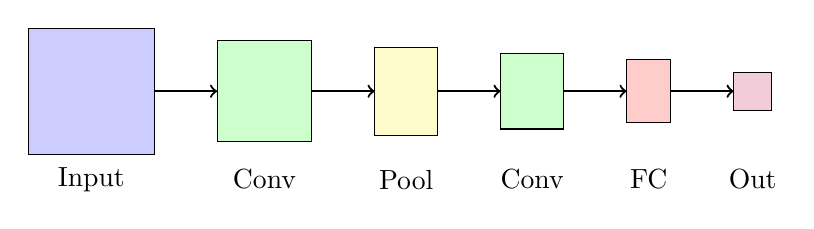
\begin{tikzpicture}[scale=0.8]
    % Input
    \draw[fill=blue!20] (0,0) rectangle (2,2);
    \node at (1,-0.4) {Input};
    
    % Conv1
    \draw[fill=green!20] (3,0.2) rectangle (4.5,1.8);
    \node at (3.75,-0.4) {Conv};
    
    % Pool1
    \draw[fill=yellow!20] (5.5,0.3) rectangle (6.5,1.7);
    \node at (6,-0.4) {Pool};
    
    % Conv2
    \draw[fill=green!20] (7.5,0.4) rectangle (8.5,1.6);
    \node at (8,-0.4) {Conv};
    
    % FC
    \draw[fill=red!20] (9.5,0.5) rectangle (10.2,1.5);
    \node at (9.85,-0.4) {FC};
    
    % Output
    \draw[fill=purple!20] (11.2,0.7) rectangle (11.8,1.3);
    \node at (11.5,-0.4) {Out};
    
    % Arrows
    \draw[->, thick] (2,1) -- (3,1);
    \draw[->, thick] (4.5,1) -- (5.5,1);
    \draw[->, thick] (6.5,1) -- (7.5,1);
    \draw[->, thick] (8.5,1) -- (9.5,1);
    \draw[->, thick] (10.2,1) -- (11.2,1);
\end{tikzpicture}
\caption{Kiến trúc CNN cơ bản}
\label{fig:cnn_arch}
\end{figure}

\subsection{Phép tích chập (Convolution)}

Phép tích chập 2D giữa input $I$ và kernel $K$ kích thước $m \times n$ được định nghĩa:

\begin{equation}
(I * K)(i,j) = \sum_{p=0}^{m-1} \sum_{q=0}^{n-1} I(i+p, j+q) \cdot K(p,q)
\label{eq:convolution}
\end{equation}

Kernel ``trượt'' qua toàn bộ ảnh, tạo ra feature map mới. Các kernel khác nhau trích xuất các đặc trưng khác nhau: cạnh, góc, kết cấu, v.v.

\subsection{Các thành phần chính}

\begin{itemize}
    \item \textbf{Convolutional Layer}: Áp dụng nhiều filter để trích xuất đặc trưng.
    \item \textbf{Pooling Layer}: Giảm kích thước spatial, tăng tính bất biến với dịch chuyển. Phổ biến nhất là Max Pooling.
    \item \textbf{Activation Function}: ReLU, Leaky ReLU, SiLU (Swish) --- thêm tính phi tuyến.
    \item \textbf{Batch Normalization}: Chuẩn hóa output theo batch, ổn định quá trình training.
    \item \textbf{Fully Connected Layer}: Kết nối toàn phần ở cuối mạng để phân loại.
\end{itemize}

\section{Kiến trúc YOLO (You Only Look Once)}

\subsection{Lịch sử phát triển}

\Gls{yolo} được giới thiệu lần đầu bởi Redmon et al. (2016) với ý tưởng đột phá: coi object detection như một bài toán hồi quy đơn lẻ, dự đoán bounding box và class probability trong một lần forward pass. Đây là bước nhảy vọt so với các phương pháp 2-stage như R-CNN.

\begin{table}[H]
\centering
\caption{Tiến hóa của kiến trúc YOLO}
\label{tab:yolo_evolution}
\begin{tabular}{@{}lllp{5cm}@{}}
\toprule
\textbf{Version} & \textbf{Năm} & \textbf{Tác giả} & \textbf{Đặc điểm nổi bật} \\
\midrule
YOLOv1 & 2016 & Redmon et al. & Ý tưởng one-stage đầu tiên \\
YOLOv2 & 2017 & Redmon et al. & Batch Norm, anchor boxes \\
YOLOv3 & 2018 & Redmon et al. & Multi-scale detection \\
YOLOv4 & 2020 & Bochkovskiy et al. & CSPDarknet, PANet \\
YOLOv5 & 2020 & Ultralytics & PyTorch, model scaling \\
YOLOv8 & 2023 & Ultralytics & Anchor-free, SOTA accuracy \\
YOLO11 & 2024 & Ultralytics & Optimized efficiency \\
\bottomrule
\end{tabular}
\end{table}

\subsection{YOLOv8 --- Kiến trúc sử dụng trong đề tài}

YOLOv8 (Ultralytics, 2023) là phiên bản mới nhất tại thời điểm thực hiện đề tài, với các cải tiến chính:

\begin{itemize}
    \item \textbf{Anchor-free detection}: Loại bỏ anchor boxes, đơn giản hóa thiết kế.
    \item \textbf{C2f module}: Kết hợp CSP (Cross Stage Partial) với ELAN, tăng gradient flow.
    \item \textbf{Decoupled head}: Tách riêng classification và regression head.
    \item \textbf{Unified API}: Hỗ trợ detection, segmentation, classification, pose trong cùng framework.
\end{itemize}

\begin{figure}[H]
\centering
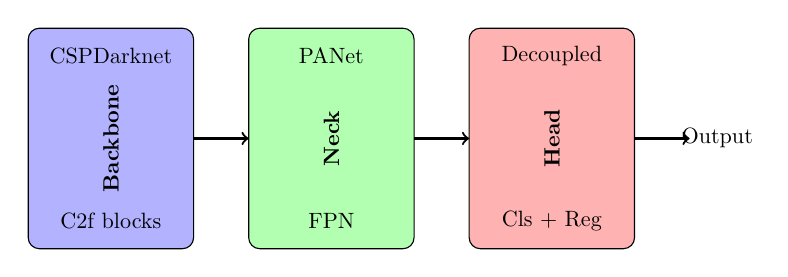
\begin{tikzpicture}[scale=0.7, every node/.style={scale=0.8}]
    % Backbone
    \draw[fill=blue!30, rounded corners] (0,0) rectangle (3,4);
    \node[rotate=90] at (1.5,2) {\textbf{Backbone}};
    \node at (1.5,3.5) {CSPDarknet};
    \node at (1.5,0.5) {C2f blocks};
    
    % Neck
    \draw[fill=green!30, rounded corners] (4,0) rectangle (7,4);
    \node[rotate=90] at (5.5,2) {\textbf{Neck}};
    \node at (5.5,3.5) {PANet};
    \node at (5.5,0.5) {FPN};
    
    % Head
    \draw[fill=red!30, rounded corners] (8,0) rectangle (11,4);
    \node[rotate=90] at (9.5,2) {\textbf{Head}};
    \node at (9.5,3.5) {Decoupled};
    \node at (9.5,0.5) {Cls + Reg};
    
    % Arrows
    \draw[->, thick] (3,2) -- (4,2);
    \draw[->, thick] (7,2) -- (8,2);
    \draw[->, thick] (11,2) -- (12,2);
    \node at (12.5,2) {Output};
\end{tikzpicture}
\caption{Kiến trúc tổng quan YOLOv8}
\label{fig:yolov8_arch}
\end{figure}

\subsection{YOLOv8 Classification Mode}

Ngoài detection, YOLOv8 còn hỗ trợ \textbf{classification mode} (yolov8n-cls.pt), trong đó:
\begin{itemize}
    \item Backbone trích xuất đặc trưng từ toàn bộ ảnh.
    \item Global Average Pooling tổng hợp feature map.
    \item Fully Connected Layer dự đoán xác suất từng class.
\end{itemize}

Đây là mode được sử dụng cho classifier trong pipeline của đề tài.

\section{Không gian màu và phân tích màu sắc}

\subsection{Không gian màu RGB}

RGB (Red-Green-Blue) là không gian màu phổ biến nhất trong hình ảnh số, với mỗi pixel được biểu diễn bởi 3 thành phần:

\begin{equation}
\text{Pixel} = (R, G, B), \quad R, G, B \in [0, 255]
\end{equation}

Tuy nhiên, RGB không phù hợp cho phân tích màu sắc vì:
\begin{itemize}
    \item Các kênh có tương quan cao, khó tách riêng thông tin màu.
    \item Nhạy cảm với điều kiện chiếu sáng.
\end{itemize}

\subsection{Không gian màu HSV}

\Gls{hsv} tách riêng thông tin màu sắc (Hue), độ bão hòa (Saturation) và độ sáng (Value):

\begin{equation}
\text{HSV} = (H, S, V), \quad H \in [0, 180], \; S, V \in [0, 255]
\end{equation}

Trong đề tài, chúng tôi sử dụng HSV để định nghĩa các ngưỡng màu cho chuối:

\begin{table}[H]
\centering
\caption{Ngưỡng HSV cho phân loại màu chuối}
\label{tab:hsv_thresholds}
\begin{tabular}{@{}lcc@{}}
\toprule
\textbf{Màu sắc} & \textbf{HSV thấp} & \textbf{HSV cao} \\
\midrule
Vàng (chín) & (15, 80, 80) & (35, 255, 255) \\
Xanh (xanh) & (35, 40, 40) & (85, 255, 255) \\
Nâu (quá chín) & (5, 50, 20) & (20, 200, 150) \\
Đen (hỏng) & (0, 0, 0) & (180, 255, 50) \\
\bottomrule
\end{tabular}
\end{table}

\subsection{Không gian màu LAB}

\Gls{lab} (CIE L*a*b*) được thiết kế để gần với nhận thức màu của mắt người:
\begin{itemize}
    \item $L^*$: Lightness (độ sáng), [0, 100]
    \item $a^*$: Green-Red axis
    \item $b^*$: Blue-Yellow axis
\end{itemize}

LAB được sử dụng trong đề tài cho:
\begin{itemize}
    \item \textbf{\Gls{clahe}}: Tăng cường độ tương phản trên kênh L.
    \item \textbf{Color uniformity}: Tính độ đồng đều màu sắc qua độ lệch chuẩn.
\end{itemize}

\section{Các kỹ thuật xử lý ảnh}

\subsection{Morphological Operations}

Các phép toán hình thái học thao tác trên hình dạng của đối tượng trong ảnh nhị phân:

\begin{itemize}
    \item \textbf{Erosion}: Co nhỏ đối tượng, loại bỏ noise nhỏ.
    \item \textbf{Dilation}: Mở rộng đối tượng, lấp đầy lỗ hổng.
    \item \textbf{Opening}: Erosion $\rightarrow$ Dilation, loại noise.
    \item \textbf{Closing}: Dilation $\rightarrow$ Erosion, lấp lỗ.
\end{itemize}

\subsection{Contour Analysis}

Contour (đường viền) của đối tượng cung cấp thông tin hình thái quan trọng:

\begin{equation}
\text{Solidity} = \frac{\text{Area}}{\text{Convex Hull Area}}
\end{equation}

\begin{equation}
\text{Aspect Ratio} = \frac{\text{Width}}{\text{Height}}
\end{equation}

Các đặc trưng này giúp phân biệt chuối lành (solidity cao, hình dạng đều) với chuối hỏng (bề mặt không đều).

\subsection{Texture Analysis}

Kết cấu bề mặt được đo bằng \textbf{Laplacian variance}:

\begin{equation}
\text{Texture Variance} = \text{Var}(\nabla^2 I)
\end{equation}

trong đó $\nabla^2 I$ là Laplacian của ảnh grayscale. Giá trị cao chỉ ra bề mặt gồ ghề (có thể do đốm, vết thối).

\section{Đánh giá mô hình}

\subsection{Confusion Matrix}

Ma trận nhầm lẫn (Confusion Matrix) là công cụ cơ bản để đánh giá mô hình phân loại. Nó cung cấp cái nhìn chi tiết về số lượng mẫu được phân loại đúng/sai cho từng class, giúp xác định các \textit{kiểu lỗi} của mô hình. Với bài toán 4 class (unripe/ripe/overripe/rotten), confusion matrix 4$\times$4 cho phép phân tích xem mô hình có học được ``thứ tự chín'' hay không --- nếu các nhầm lẫn chỉ xảy ra giữa các class liền kề, đó là dấu hiệu tích cực.

Với nền tảng lý thuyết này, chương tiếp theo sẽ trình bày \textbf{phương pháp thực hiện} --- cách chúng tôi thiết kế hệ thống dựa trên các khái niệm đã giới thiệu.

\clearpage

\begin{table}[H]
\centering
\caption{Cấu trúc Confusion Matrix cho 2 lớp}
\label{tab:confusion_matrix}
\begin{tabular}{@{}l|cc@{}}
\toprule
& \textbf{Predicted Positive} & \textbf{Predicted Negative} \\
\midrule
\textbf{Actual Positive} & True Positive (TP) & False Negative (FN) \\
\textbf{Actual Negative} & False Positive (FP) & True Negative (TN) \\
\bottomrule
\end{tabular}
\end{table}

\subsection{Các chỉ số đánh giá}

\begin{itemize}
    \item \textbf{Accuracy}:
    \begin{equation}
    \text{Accuracy} = \frac{TP + TN}{TP + TN + FP + FN}
    \end{equation}
    
    \item \textbf{Precision} (độ chính xác):
    \begin{equation}
    \text{Precision} = \frac{TP}{TP + FP}
    \end{equation}
    
    \item \textbf{Recall} (độ phủ):
    \begin{equation}
    \text{Recall} = \frac{TP}{TP + FN}
    \end{equation}
    
    \item \textbf{F1-Score}:
    \begin{equation}
    F_1 = 2 \cdot \frac{\text{Precision} \cdot \text{Recall}}{\text{Precision} + \text{Recall}}
    \end{equation}
\end{itemize}

Trong bài toán phân loại chuối hỏng, \textbf{Recall cho class ``defective'' đặc biệt quan trọng}: chúng ta muốn phát hiện được tất cả chuối hỏng (ít false negative), thà loại nhầm còn hơn bỏ sót.

\subsection{Top-1 và Top-5 Accuracy}

Trong classification, ngoài accuracy tiêu chuẩn, ta còn đánh giá:
\begin{itemize}
    \item \textbf{Top-1 Accuracy}: Tỉ lệ mẫu mà class dự đoán cao nhất đúng.
    \item \textbf{Top-5 Accuracy}: Tỉ lệ mẫu mà class đúng nằm trong top 5 dự đoán.
\end{itemize}

\section{Tóm tắt chương}

Chương này đã trình bày nền tảng lý thuyết cho hệ thống phân loại chất lượng chuối:
\begin{itemize}
    \item \textbf{Thị giác máy tính} và các bài toán cơ bản (detection, classification).
    \item \textbf{Mạng nơ-ron tích chập (CNN)} với các nguyên lý: local connectivity, weight sharing, hierarchical compositionality.
    \item \textbf{Kiến trúc YOLO} và sự tiến hóa từ v1 đến v8, đặc biệt là YOLOv8 classification mode.
    \item \textbf{Không gian màu HSV/LAB} và ứng dụng trong phân tích màu sắc chuối.
    \item \textbf{Các metrics đánh giá}: Confusion Matrix, Accuracy, Precision, Recall, F1-Score.
\end{itemize}

Với nền tảng lý thuyết này, chương tiếp theo sẽ trình bày \textbf{phương pháp thực hiện} --- cách chúng tôi thiết kế hệ thống 2-stage pipeline dựa trên các khái niệm đã giới thiệu.

\clearpage
